\chapter{Θεωρητικό Υπόβαθρο} \label{chap:correlations}
\section{Συσχετίσεις}
\subsection{Ορισμός}
\paragraph*{}
Η έννοια των συσχετίσεων (correlations) χρησιμοποιείται κατά κόρον στην επεξεργασία σήματος και εικόνας. Έστω $x(\textbf{t})$ ένα διακριτό σήμα δύο διαστάσεων (\textbf{2D}), όπου $\boldsymbol{t}\in S = [0, \cdots ,N-1]\times[0, \cdots ,N-1]$. Η συσχέτιση δεύτερης και τρίτης τάξης αυτού του σήματος ορίζεται ως:

\begin{equation} \label{eq:corr22}
x_2(\boldsymbol{\tau})  \triangleq \sum\limits_{\boldsymbol{t}\in S}x(\boldsymbol{t})x(\boldsymbol{t}+\boldsymbol{\tau}) 
\end{equation}
\begin{equation} \label{eq:corr23}
x_3(\boldsymbol{\tau_1},\boldsymbol{\tau_2}) \triangleq \sum\limits_{\boldsymbol{t}\in S}x(\boldsymbol{t})x(\boldsymbol{t}+\boldsymbol{\tau_1}) x(\boldsymbol{t}+\boldsymbol{\tau_2}) 
\end{equation}
αντίστοιχα, όπου $\boldsymbol{\tau}, \boldsymbol{\tau_1}, \boldsymbol{\tau_2} \in S'=[-(N-1), \cdots ,N-1]\times[-(N-1), \cdots ,N-1]$.
\paragraph*{}
Οι παραπάνω εξισώσεις (\ref{eq:corr22} και \ref{eq:corr23}) αφορούν σε ντετερμινιστικά σήματα. Στην περίπτωση των στοχαστικών σημάτων γίνεται χρήση των εκτιμητριών συναρτήσεων υπολογισμού ροπών:
\begin{equation}
m_2^N(\boldsymbol{\tau}) \triangleq \dfrac{1}{N} \sum\limits_{\boldsymbol{t}\in S}x(\boldsymbol{t})x(\boldsymbol{t}+\boldsymbol{\tau})
\end{equation}
\begin{equation}
m_3^N(\boldsymbol{\tau_1},\boldsymbol{\tau_2}) \triangleq \dfrac{1}{N^2} \sum\limits_{\boldsymbol{t}\in S}x(\boldsymbol{t})x(\boldsymbol{t}+\boldsymbol{\tau_1}) x(\boldsymbol{t}+\boldsymbol{\tau_2})
\end{equation}
όπου και πάλι $\boldsymbol{\tau}, \boldsymbol{\tau_1}, \boldsymbol{\tau_2} \in S'=[-(N-1), \cdots ,N-1]\times[-(N-1), \cdots ,N-1]$.

\paragraph*{}
Οι παραπάνω τύποι υπολογίζουν τις συσχετίσεις διδιάστατων σημάτων. Αντίστοιχα μπορούν να υπολογισθούν οι συσχετίσεις μονοδιάστατων (\textbf{1D}) σημάτων. Έστω $x(t)$ ένα διακριτό μονοδιάστατο σήμα, όπου $t \in S = [0, \cdots ,N-1]$:

\begin{equation} 
x_2(\tau) \triangleq \sum\limits_{t \in S} x(t)x(t+\tau) 
\end{equation}
\begin{equation} 
x_3(\tau_1,\tau_2) \triangleq \sum\limits_{t \in S}x (t)x(t+\tau_1) x(t+\tau_2) 
\end{equation}
\begin{equation}
m_2^N(\tau) \triangleq \dfrac{1}{N} \sum\limits_{t \in S}x (t)x(t+\tau)
\end{equation}
\begin{equation}
m_3^N(\tau_1,\tau_2) \triangleq \dfrac{1}{N^2} \sum\limits_{t \in S}x(t) x(t+\tau_1)x(t+\tau_2)
\end{equation}
όπου $\tau, \tau_1, \tau_2 \in S'=[-(N-1), \cdots ,N-1]$.

\paragraph*{}
Στην περίπτωση, λοιπόν ενός διδιάστατου διακριτού σήματος, δηλαδή μίας εικόνας, η συσχέτιση τρίτου βαθμού υπολογίζεται από την εξίσωση \ref{eq:corr23}. Αυτό θα χρησιμοποιηθεί στα πλαίσια της παρούσας διπλωματικής εργασίας. Θα πρέπει να σημειωθεί πως το αποτέλεσμα της εξίσωσης \ref{eq:corr23} είναι ένας πίνακας τεσσάρων διαστάσεων (\textbf{4D}), με κάθε διάσταση να έχει μήκος $(2 \times N - 1)$.
\paragraph*{}
Οι παραπάνω σχέσεις ισχύουν για τετραγωνικά\footnote{Τετραγωνικά χαρακτηρίζονται τα σήματα δύο διαστάσεων, των οποίων και οι δύο διαστάσεις έχουν ίδιο μήκος.}  και μη σήματα. Για λόγους απλότητας όμως, θεωρούμε στο εξής πως τα σήματα με τα οποία ασχολούμαστε είναι τετραγωνικά. Άλλωστε κάτι τέτοιο δεν είναι δύσκολο να ισχύει, αφού στην περίπτωση που έχουμε ένα μη τετραγωνικό σήμα, αυτό μπορεί εύκολα να μετατραπεί σε τετραγωνικό με επέκταση της μικρότερης διάστασης.


% ===========================================================================================================================
% ===========================================================================================================================

\subsection{Ιδιότητες των Συσχετίσεων} \label{sec:properties}
Σε αυτό το κομμάτι θα αναλυθούν κάποιες ενδιαφέρουσες και πολύ χρήσιμες ιδιότητες των συσχετίσεων. Έστω ένα διδιάστατο διακριτό ντετερμινιστικό σήμα $x(\textbf{t}),\textbf{t}\in S = [0, \cdots ,N-1]\times[0, \cdots ,N-1]$, διάστασης $N \times N$. Έστω η συσχέτιση δεύτερης και τρίτης τάξης $x_2(\boldsymbol{\tau})$ και $x_3(\boldsymbol{\tau_1},\boldsymbol{\tau_2}), \boldsymbol{\tau}, \boldsymbol{\tau_1}, \boldsymbol{\tau_2} \in S'=[-(N-1), \cdots ,N-1]\times[-(N-1), \cdots ,N-1]$, που υπολογίσθηκαν από τις εξισώσεις \ref{eq:corr22} και \ref{eq:corr23} αντίστοιχα.
\paragraph*{Συμμετρίες}
Ισχύουν οι παρακάτω σχέσεις συμμετρίας:
\begin{align}
x_2(\boldsymbol{\tau}) = x_2(-\boldsymbol{\tau})
\end{align}

\begin{align} \label{eq:symmetries}
 x_3(\boldsymbol{\tau_1},\boldsymbol{\tau_2}) &= x_3(\boldsymbol{\tau_1}-\boldsymbol{\tau_2},-\boldsymbol{\tau_2}) = x_3(\boldsymbol{\tau_2}-\boldsymbol{\tau_1},-\boldsymbol{\tau_1}) \nonumber\\
    &= x_3(\boldsymbol{\tau_2},\boldsymbol{\tau_1}) = x_3(-\boldsymbol{\tau_1},\boldsymbol{\tau_2}-\boldsymbol{\tau_1}) \\
    &= x_3(-\boldsymbol{\tau_2},\boldsymbol{\tau_1}-\boldsymbol{\tau_2})  \nonumber 
\end{align}
\\Οι συμμετρίες αυτές ισχύουν και για μονοδιάστατα και για στοχαστικά σήματα και είναι πολύ χρήσιμες στην υλοποίηση των συναρτήσεων που υπολογίζουν τις συσχετίσεις, καθώς μπορούν να μειώσουν την υπολογιστική πολυπλοκότητα και τη μνήμη που χρειάζεται για να αποθηκευθούν τα αποτελέσματα.

\paragraph*{Αναισθησία στο θόρυβο}
Έστω $e(\boldsymbol{t})$ Gaussian θόρυβος με μηδενική μέση τιμή ή γραμμικός και συμμετρικά κατανεμημένος θόρυβος. Ισχύει:
\begin{equation}
E\lbrace e_3(\boldsymbol{\tau_1},\boldsymbol{\tau_2})\rbrace=0
\end{equation}
Επίσης ισχύει:
\begin{equation}
e_3(\boldsymbol{\tau_1},\boldsymbol{\tau_2}) \rightarrow 0 \textrm{ αν } N \rightarrow \infty
\end{equation}
\\Έστω $y(\textbf{t})= x(\textbf{t})+e(\textbf{t})$, το αρχικό διδιάστατο σήμα παραμορφωμένο από θόρυβο. Τότε έχουμε:
\begin{equation}
E \lbrace y_3(\boldsymbol{\tau_1},\boldsymbol{\tau_2}) \rbrace = x_3(\boldsymbol{\tau_1},\boldsymbol{\tau_2}), \forall (\boldsymbol{\tau_1},\boldsymbol{\tau_2})
\end{equation}
\\Η αναμενόμενη τιμή της συσχέτισης του παραμορφωμένου σήματος είναι ανεξάρτητη του θορύβου.\\
Σε γενικές γραμμές, υπό συνθήκες που εξασφαλίζουν την ύπαρξη του $x_3(\boldsymbol{\tau_1},\boldsymbol{\tau_2})$, θεωρείται πως $y_3(\boldsymbol{\tau_1},\boldsymbol{\tau_2}) = x_3(\boldsymbol{\tau_1},\boldsymbol{\tau_2})$.

\paragraph*{1-1 Αντιστοιχία}
Δεδομένου ότι $x_3(\boldsymbol{\tau_1},\boldsymbol{\tau_2})\neq 0$, δηλαδή \textbf{τουλάχιστον ένα} στοιχείο της συσχέτισης δεν είναι μηδενικό, υπάρχει μία 1-1 αντιστοιχία μεταξύ του διδιάστατου σήματος και της συσχέτισής του:
\begin{equation}
x_3(\boldsymbol{\tau_1},\boldsymbol{\tau_2}) = y_3(\boldsymbol{\tau_1},\boldsymbol{\tau_2}) \Leftrightarrow x(\textbf{t})=y(\textbf{t})
\end{equation}
\\Αυτό σημαίνει πως, κατά τον υπολογισμό των συσχετίσεων τρίτης τάξης, δεν υπάρχει απώλεια πληροφορίας του σήματος. Μπορούμε, δηλαδή, να αναγνωρίσουμε το σήμα από τη συσχέτισή του.

\paragraph*{Μεταφορά - Περιστροφή - Κλιμάκωση}
Έστω $y(\textbf{t}) = x(\textbf{T}_{\alpha,\theta}\textbf{t}+\textbf{t}_0)$, όπου:

\begin{equation}
\textbf{T}_{\alpha,\theta} = \alpha 
\begin{bmatrix} \cos\theta & -\sin\theta \\ \sin\theta & \cos\theta \end{bmatrix}
\end{equation}
πίνακας περιστροφής περί την αρχή των αξόνων κατά γωνία θ και διαστολής / συστολής κατά α και $\textbf{t}_0$ διάνυσμα μετατόπισης. Δεδομένου ότι μπορεί να εφαρμοστεί αυτός ο μετασχηματισμός, ισχύει:
\begin{equation}\label{eq:rot}
y_3(\boldsymbol{\tau_1},\boldsymbol{\tau_2}) = x(\textbf{T}_{\alpha,\theta}\boldsymbol{\tau_1},\textbf{T}_{\alpha,\theta}\boldsymbol{\tau_1})
\end{equation}
Αυτό σημαίνει πως οι συσχετίσεις δεν επηρεάζονται από τη μετατόπιση του αρχικού σήματος. Όσον αφορά στην περιστροφή και/ή κλιμάκωση, όπως φαίνεται από την εξίσωση \ref{eq:rot}, ένας αντίστοιχος μετασχηματισμός εφαρμόζεται και στα δυο διανύσματα-δείκτες της συσχέτισης.\\
Εν ολίγοις αν το αρχικό σήμα περιστραφεί ή/και κλιμακωθεί, τότε το περιεχόμενο της συσχέτισής του δεν αλλάζει, αλλά αλλάζουν θέση τα στοιχεία του. Αν λοιπόν γνωρίζουμε τη γωνία περιστροφής ή/και το λόγο κλιμάκωσης, τότε μπορούμε να γνωρίζουμε τις νέες θέσεις των στοιχείων αυτών.\\
\textit{Σημείωση: }Η παραπάνω ιδιότητα ισχύει δεδομένου ότι μετά το μετασχηματισμό του αρχικού σήματος δεν υπάρχει απώλεια πληροφορίας. Μπορούμε, δηλαδή να θεωρήσουμε πως το $x(\textbf{t})$ είναι αρχικά τοποθετημένο πάνω σε ένα πλαίσιο $P = [0, \cdots ,M-1]\times[0, \cdots ,M-1], M>N$. Η απαίτησή μας για να ισχύει η ιδιότητα, είναι, πως μετά τον οποιοδήποτε μετασχηματισμό που θα υποστεί το σήμα, θα βρίσκεται ολόκληρο στο εσωτερικό του $P$. Για αυτό το λόγο κάνουμε εξ' αρχής την παραδοχή, ότι το $S$ έχει τέτοιο μέγεθος, ώστε να υπάρχει το περιθώριο για το $x(\textbf{t})$ να μετασχηματιστεί, χωρίς να υποστεί αποκοπή στις άκρες του.


% ===========================================================================================================================
% ===========================================================================================================================

\subsection{Συσχετίσεις \& Μετασχηματισμός Fourier}
Η σημαντικότερη, ίσως, ιδιότητα των συσχετίσεων, είναι αυτή που τις συνδέει με το μετασχηματισμό Fourier. Έστω $x(\textbf{t}), x_2(\boldsymbol{\tau})$ και $x_3(\boldsymbol{\tau_1},\boldsymbol{\tau_2})$ το αρχικό σήμα και οι συσχετίσεις του, όπως στην παράγραφο \ref{sec:properties}.
\paragraph*{}
Αν $X(\boldsymbol{\omega}), X_2(\boldsymbol{\omega})$ και $X_3(\boldsymbol{\omega_1},\boldsymbol{\omega_2})$ οι μετασχηματισμοί Fourier των $x(\textbf{t}), x_2(\boldsymbol{\tau})$ και $x_3(\boldsymbol{\tau_1},\boldsymbol{\tau_2})$ αντίστοιχα, οι οποίοι υπολογίζονται από τον τύπο του διακριτού μετασχηματισμού Fourier:
\begin{equation}
F(k,l) = \sum_{i=0}^{N-1}\sum_{j=0}^{N-1}f(i,j)e^{-i2\pi\left(\frac{ki}{N}+\frac{lj}{N}\right)}
\end{equation}
τότε, εύκολα με πράξεις, αποδεικνύεται πως ισχύουν οι παρακάτω δύο ιδιότητες:
\begin{equation} \label{eq:dft22}
X_2(\boldsymbol{\omega}) = |X(\boldsymbol{\omega})|^2 = X(\boldsymbol{\omega})X^*(\boldsymbol{\omega}) = X(\boldsymbol{\omega})X(-\boldsymbol{\omega})
\end{equation}
\begin{equation}\label{eq:dft23}
X_3(\boldsymbol{\omega_1},\boldsymbol{\omega_2}) = X(\boldsymbol{\omega_1})X(\boldsymbol{\omega_2})X(-\boldsymbol{\omega_1} -\boldsymbol{\omega_2}) = X(\boldsymbol{\omega_1})X(\boldsymbol{\omega_2})X^*(\boldsymbol{\omega_1} +\boldsymbol{\omega_2})
\end{equation}
\\Οι ιδιότητες αυτές μας δείχνουν πως μπορούμε να υπολογίσουμε τους μετασχηματισμούς Fourier των συσχετίσεων, απλά και μόνο γνωρίζοντας το μετασχηματισμό Fourier του σήματος. Μπορούμε, δηλαδή να υπολογίσουμε τις ίδιες τις συσχετίσεις (μέσω του αντίστροφου μετασχηματισμού Fourier) γνωρίζοντας μόνο το μετασχηματισμό Fourier του αρχικού σήματος. Αυτό είναι πάρα πολύ χρήσιμο υπολογιστικά, καθώς μας συμφέρει, από άποψη πολυπλοκότητας κώδικα και από άποψη χρόνου, να βρίσκουμε τις συσχετίσεις, μέσω αυτής της ιδιότητας, με τη χρήση έτοιμων συναρτήσεων υπολογισμού ευθύ και αντίστροφου μετασχηματισμού Fourier, παρά με τη χρήση του ορισμού τους (εξισώσεις \ref{eq:corr22} και \ref{eq:corr23}).
\paragraph*{}
Ιδιαίτερα ενδιαφέρον είναι το γεγονός ότι, μέσω της ιδιότητας \ref{eq:dft23}, μπορούμε να υπολογίσουμε το αρχικό σήμα γνωρίζοντας την τρίτης τάξης συσχέτισή του (ή το μετασχηματισμό Fourier της). Το ίδιο, όμως, δε συμβαίνει μέσω της ιδιότητας \ref{eq:dft22}, αφού η ιδιότητα αυτή συνδέει το μετασχηματισμό Fourier της δεύτερης τάξης συσχέτισης με το μέτρο του μετασχηματισμού Fourier του αρχικού σήματος. Σε αυτή την περίπτωση, δηλαδή, δεν υπάρχει 1-1 αντιστοιχία.

% ===========================================================================================================================
% ===========================================================================================================================

%\section{Γκαουσιανή Συνάρτηση} \label{sec:gaussian}
%\paragraph*{}
%Η γκαουσιανή συνάρτηση (Gaussian Function) ορίζεται από τον τύπο:
%\begin{equation}
%f(x) = \alpha e^{-\dfrac{(x-\mu)^2}{2\sigma^2}}
%\end{equation}
%όπου $\alpha,\mu,\sigma \in \mathbf{R}$. Το γράφημα της γκαουσιανής συνάρτησης έχει το σχήμα καμπάνας ("bell curve") (Σχ. \ref{fig:bell}), είναι δηλαδή συμμετρικό και τείνει προς το μηδέν ασυμπτωτικά. Το $\alpha$ ορίζει το ύψος της καμπύλης, το $\mu$ ορίζει το που θα βρίσκεται ο κεντρικός άξονας συμμετρίας και το $\sigma$ (τυπική απόκλιση) το πλάτος της "καμπάνας". Όπως φαίνεται και στο Σχήμα \ref{fig:bell}, όσο πιο μικρο είναι το $\sigma$, τόσο πιο κοντά στο κέντρο της καμπύλης φτάνουμε σε σχεδόν μηδενικές τιμές. Ιδιαίτερα χρήσιμη είναι η πληροφορία που παίρνουμε από το Σχήμα \ref{fig:distribution}. Αυτό που φαίνεται στο σχήμα είναι, πως σε απόσταση $3\sigma$ συμμετρικά του κέντρου της καμπύλης συγκεντρώνεται το 99.8\% της πληροφορίας της συνάρτησης.
%
%\begin{figure}[!b]
%\centerline{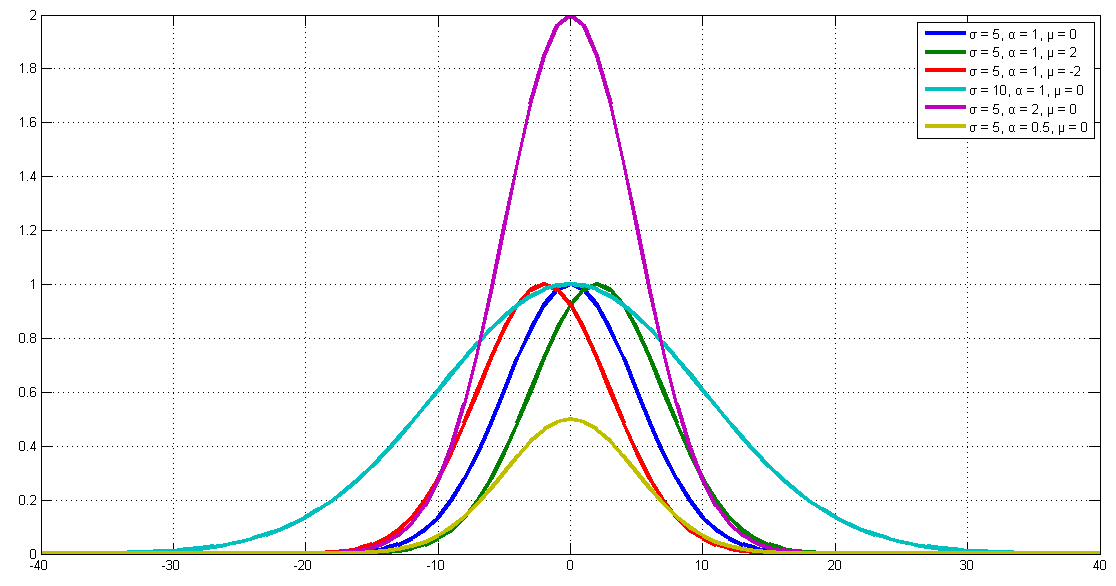
\includegraphics[scale=0.6]{./images/gaussianCurves.png}}
%\caption{Γραφήματα της Γκαουσιανής συνάρτησης για διάφορα $\alpha,\mu$ και $\sigma$}
%\label{fig:bell}
%\end{figure}
%
%\begin{figure}
%\centerline{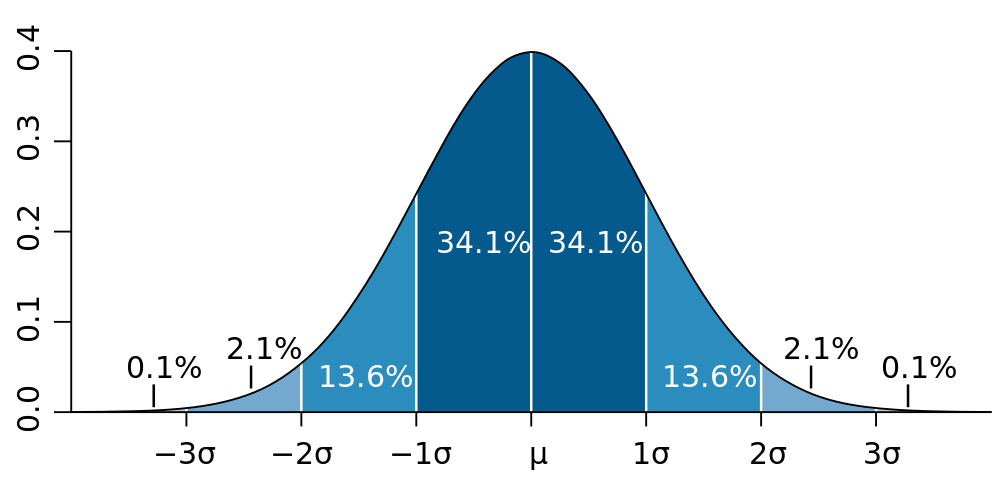
\includegraphics[scale=0.3]{./images/gaussianLarge.png}}
%\caption{Κατανομή της καμπύλης της Γκαουσιανής συνάρτησης}
%\label{fig:distribution}
%\end{figure}
%
%\paragraph*{}
%Η γκαουσιανή συνάρτηση ορίζεται και για δύο διαστάσεις. Ο τύπος για τη διδιάστατη γκαουσιανή συνάρτηση είναι:
%\begin{equation}
%f(x,y) = \alpha e^{-\left(\dfrac{(x-x_0)^2}{2\sigma_x^2}+\dfrac{(y-y_0)^2}{2\sigma_y^2}\right)}
%\end{equation}
%\begin{wrapfigure}{r}{0.3\textwidth}
%\centerline{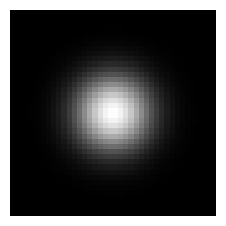
\includegraphics[scale=0.25]{./images/gauss2DImage.png}}
%\caption{Γκαουσιανή συνάρτηση ως εικόνα}
%\label{fig:2dbellimage}
%\end{wrapfigure}
%όπου $\alpha, x_0, y_0,\sigma_x, \sigma_y \in \mathbf{R}$. Αντίστοιχα με την γκαουσιανή στη μία διάσταση, το γράφημα στις δυο διαστάσεις έχει και πάλι το σχήμα καμπάνας (Σχ. \ref{fig:2dbell}). Το $\alpha$ ορίζει το ύψος την επιφάνειας, τα $(x_0,y_0)$, ορίζουν το κέντρο και τα $(\sigma_x,\sigma_y)$ ορίζουν τα πλάτη της καμπάνας ως προς τους άξονες x και y αντίστοιχα.
%
%\begin{figure}[!b]
%\centerline{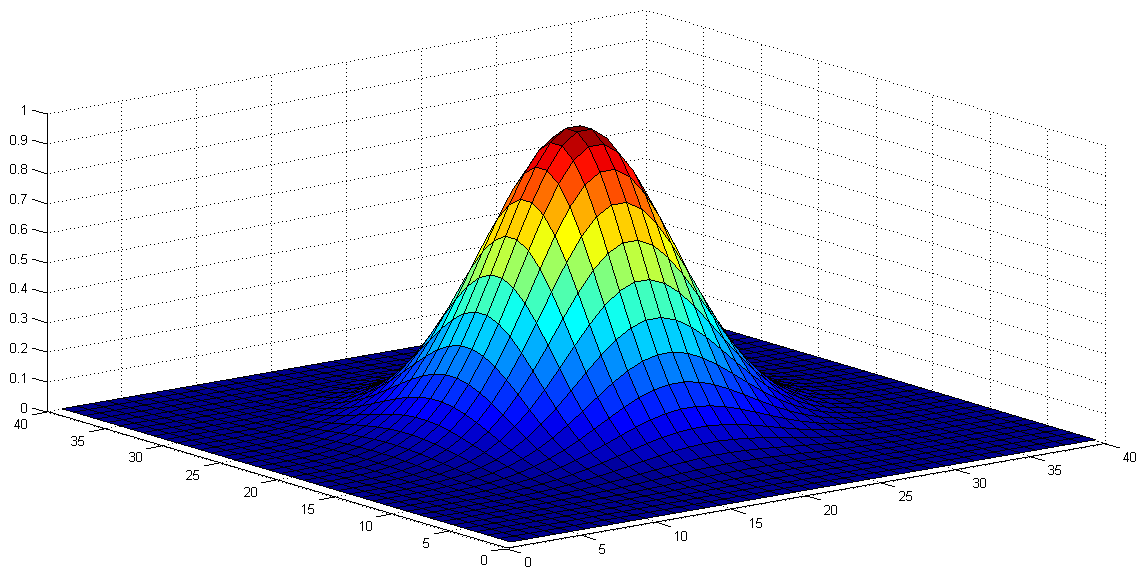
\includegraphics[scale=0.35]{./images/gauss2DCurve.png}}
%\caption{Γράφημα της Γκαουσιανής συνάρτησης στις δύο διαστάσεις}
%\label{fig:2dbell}
%\end{figure}
%
%
%\begin{figure}[!t]
%        \centering
%        \begin{subfigure}[b]{0.5\textwidth}
%                \centerline{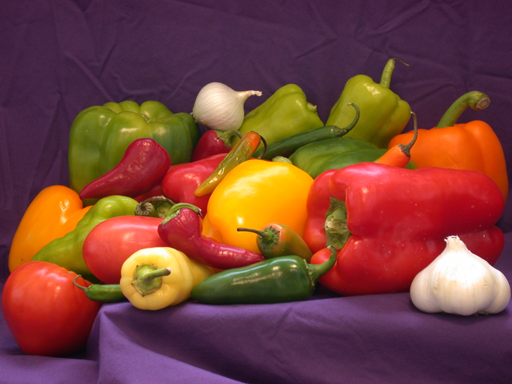
\includegraphics[scale = 0.4]{./images/peppers.png}}
%        \end{subfigure}%
%		~
%        \centering
%        \begin{subfigure}[b]{0.5\textwidth}
%                \centerline{
\includegraphics[scale = 0.4]{./images/peppers1.png}}
%        \end{subfigure}%
%
%
%        \centering
%        \begin{subfigure}[t]{0.5\textwidth}
%                \centerline{
\includegraphics[scale = 0.4]{./images/peppers2.png}}
%        \end{subfigure}%
%        ~
%        \centering
%        \begin{subfigure}[t]{0.5\textwidth}
%                \centerline{
\includegraphics[scale = 0.4]{./images/peppers4.png}}
%        \end{subfigure}%
%        \caption{Εικόνα πολλαπλασιασμένη με γκαουσιανή συνάρτηση με διαφορετικά $\sigma_x,\sigma_y$ και $(x_0,y_0)$}
%        \label{fig:peppers}
%\end{figure}
%\paragraph*{}
%Προγραμματιστικά, όταν υπολογίζουμε την γκαουσιανή συνάρτηση στις δύο διαστάσεις, στην ουσία αυτό που υπολογίζεται είναι ένας διδιάστατος πίνακας, του οποίου το στοιχείο που αντιστοιχεί στις συντεταγμένες $(x_0,y_0)$ περιέχει την τιμή $\alpha$ και οι τιμές των υπόλοιπων στοιχείων μειώνονται όσο απομακρυνόμαστε από το $(x_0,y_0)$ ακτινικά, έως ότου φτάσουμε σε τιμές πολύ κοντά στο μηδέν. Αν τον πίνακα αυτόν τον αντιμετωπίσουμε ως εικόνα\footnote{Ο πίνακας πρέπει να υποστεί κανονικοποίηση στη μονάδα, αν $\alpha \neq 1$.}, τότε το αποτέλεσμά μας είναι μία εικόνα αποχρώσεων του γκρι (grayscale), η οποία στο σημείο $(x_0,y_0)$ έχει τη μέγιστη φωτεινότητα (λευκό χρώμα) και, καθώς απομακρυνόμαστε από το σημείο αυτό η φωτεινότητα μειώνεται σταδιακά, μέχρι να φτάσουμε σε σχεδόν μηδενική φωτεινότητα (μαύρο χρώμα) (Σχ. \ref{fig:2dbellimage}). Έχοντας, λοιπόν στη διάθεσή μας τον πίνακα της γκαουσιανής συνάρτησης, μπορούμε να πολλαπλασιάσουμε το κάθε στοιχείο του με τα στοιχεία κάποιας εικόνας (έγχρωμης ή/και grayscale) και, ανάλογα με τα επιλεγμένα $\sigma_x,\sigma_y$ και $(x_0,y_0)$, να κρατήσουμε εμφανές κάποιο κομμάτι της εικόνας "εξαφανίζοντας" σταδιακά την υπόλοιπη (Σχήμα \ref{fig:peppers}). Ιδιαίτερη προσοχή χρειάζεται στην περίπτωση έγχρωμων εικόνων, όπου θα πρέπει ο πίνακας της γκαουσιανής να πολλαπλασιαστεί ξεχωριστά με κάθε χρωματική συνιστώσα της εικόνας. Για παράδειγμα, αν χρησιμοποιείται το χρωματικό μοντέλο RGB (Red Green Blue), τότε η εικόνα αναπαρίσταται από έναν πίνακα τριών διαστάσεων. Οι δυο πρώτες διαστάσεις αφορούν στη θέση κάθε σημείου πάνω στην εικόνα και η τρίτη διάσταση (με μήκος τρία) αφορά στη χρωματική συνιστώσα. Είναι δηλαδή στην ουσία, τρεις ξεχωριστοί διδιάστατοι πίνακες ίδιας διάστασης με την εικόνα, όπου ο κάθε πίνακας περιέχει τις τιμές της κάθε ξεχωριστής χρωματικής συνιστώσας. Σε αυτήν την περίπτωση θα πρέπει ο πίνακας της γκαουσιανής συνάρτησης να πολλαπλασιαστεί ξεχωριστά με καθέναν από τους τρεις πίνακες των χρωμάτων και το αποτέλεσμα αυτών των πολλαπλασιασμών θα συνθέτει την τελική εικόνα.
%
%
